\documentclass[11pt,a4paper]{article}
\usepackage[margin=25mm]{geometry}
\usepackage{amsmath,amssymb,amsfonts,amsthm}
\usepackage{booktabs,array,makecell}
\usepackage{graphicx}
\usepackage{tikz}
\usetikzlibrary{calc,arrows.meta,patterns,decorations.pathreplacing}
\usepackage{algorithm,algpseudocode}
\usepackage{listings}
\usepackage{xcolor}
\usepackage[font=small]{caption}
\usepackage{subcaption}
\usepackage[hidelinks]{hyperref}
\usepackage{authblk}

\lstset{basicstyle=\ttfamily\footnotesize,columns=fullflexible,keepspaces=true,
        frame=single,framerule=0.3pt,rulecolor=\color{gray},language=C++,
        commentstyle=\color{gray!70!black},showstringspaces=false}

\newtheorem{proposition}{Proposition}
\newtheorem{lemma}{Lemma}
\theoremstyle{remark}
\newtheorem*{remark}{Remark}

\newcommand{\I}{\mathbb{I}}
\newcommand{\fl}{\operatorname{fl}}
\newcommand{\eps}{\mathrm{u}}
\newcommand{\e}{\mathbf{e}}
\newcommand{\chg}[1]{\textcolor{blue!70!black}{#1}}
\algrenewcommand\algorithmicfor{\textbf{for}}

\title{Siddon--Jacobs ray tracing on GPUs:\\a technical note on a consistent and accurate implementation}
\author[1]{Ander Biguri}
\author[2]{Claude}
\affil[1]{Department of Applied Mathematics and Theoretical Physics (DAMTP), University of Cambridge}
\affil[2]{Anthropic}
\date{November 2026\\[4pt]\small TIGRE technical note. Accompanies CERN/TIGRE pull request \#865 (issue \#859).}

\begin{document}
\maketitle

\begin{abstract}
This technical note documents a revision of the ray--voxel (Siddon) forward projector of the TIGRE toolbox,
for anyone implementing the incremental variant of Siddon's algorithm by Jacobs et al.\ on a GPU. The
variant, as usually implemented, has two flaws. Its published initialisation is inconsistent, in exact
arithmetic, for rays that enter the image on a voxel edge, which then are integrated one voxel off; we
characterise these rays exactly. And in single precision its incremental update accumulates rounding errors
along the ray. Both have known remedies, the initialisation of Amanatides and Woo and the direct evaluation
of crossings of Siddon's original method. We show how to apply them on a GPU at the cost of Jacobs'
traversal. The revision also makes the projector 1.4--6.5 times faster on the GPUs tested, through the
arrangement of the loop and the type of its indices. The three issues, consistency, accuracy and speed, have
independent causes, and the speed could have been obtained while keeping Jacobs' traversal; but the revised
traversal addresses all three at once, and the arrangement that makes it fast is also what makes the two fixes
free. In TIGRE the projections are about 100 times more accurate and consistent for every ray.
\end{abstract}

\noindent\textbf{Keywords:} computed tomography, forward projection, Siddon's algorithm,
ray tracing, voxel traversal, GPU, floating point.


\section{Introduction}

Iterative reconstruction in computed tomography (CT) rests on two operators, the forward
projection $A\mathbf{x}$ and the backprojection $A^T\mathbf{b}$, applied hundreds of times per
reconstruction. Ray-driven forward projectors integrate the image along each X-ray path; among
them, the exact path-length method computes, for every ray, the length of its intersection with
each voxel it crosses, i.e.\ the nonzero entries of the corresponding row of the system matrix.
Siddon's algorithm~\cite{siddon1985fast} made this practical by working in the parameter of the
ray: the ray crosses three families of equally spaced planes, so the intersection lengths are the
differences between consecutive plane crossings, at a cost proportional to the number of planes
crossed rather than to the number of voxels. Jacobs et al.~\cite{jacobs1998fast} made it faster by
replacing the sorting of crossings and the per-segment voxel index computation with an incremental
traversal, which is essentially the voxel traversal of Amanatides and Woo~\cite{amanatides1987fast}
used in computer graphics. This incremental form is the one usually implemented, and on GPUs the
implementations are much alike: one thread per ray, the image in a texture, single-precision
arithmetic, and the image processed in slabs when it does not fit in GPU memory. The TIGRE
toolbox~\cite{tigre2016,tigre2020multigpu,tigre2025v3} is one such implementation, and the one we use as
reference throughout.

This note documents what we found when an issue in TIGRE (\#859: wrong projections when the image is
split in slabs) led us to re-examine its implementation, and how we changed it. It is a technical note, not
a new method: the ingredients of the revised traversal all exist in the literature, and we say where each
comes from. Its content is:
\begin{enumerate}
\item An exact characterisation of the rays for which Jacobs' initialisation is inconsistent,
independent of floating point (Section~\ref{sec:init}). This is the cause of \#859, and it also
affects whole images.
\item An analysis of the rounding errors of the incremental update in single precision, which grow
with the number of steps (Section~\ref{sec:drift}).
\item A traversal that avoids both, combining the initialisation of Amanatides and
Woo~\cite{amanatides1987fast} with the direct evaluation of crossings of Siddon~\cite{siddon1985fast}, and
arranged for SIMT execution on GPUs (Section~\ref{sec:new}).
\item An evaluation of correctness, accuracy and speed in TIGRE, including an ablation that separates the
effect of each change on the GPU (Section~\ref{sec:results}).
\end{enumerate}
The revision also made TIGRE's projector considerably faster, for reasons unrelated to the two flaws.
Section~\ref{sec:coupling} separates the three issues: they have independent causes, but one traversal
addresses them together.
Section~\ref{sec:background} recalls both algorithms and the GPU setting, and
Section~\ref{sec:discussion} discusses why the problems went unnoticed, how other implementations deal with
them, and the limitations of this study.

\section{Background}
\label{sec:background}

\subsection{Notation}

We follow the notation of~\cite{biguri2017} (Section~4.3.1), in 3D. Coordinates are in voxel units,
with the corner of the first voxel at the origin, so that voxel $(i,j,k)$ occupies
$[i,i+1)\times[j,j+1)\times[k,k+1)$. The image has $n_x\times n_y\times n_z$ voxels, bounded by the
planes $x=0,\dots,n_x$ and likewise in $y$ and $z$. A ray goes from the source $\mathbf{p}_1$ to a
detector pixel $\mathbf{p}_2$,
\begin{equation}
\mathbf{p}(\alpha)=\mathbf{p}_1+\alpha\,\mathbf{r},\qquad \mathbf{r}=\mathbf{p}_2-\mathbf{p}_1,
\qquad \alpha\in[0,1]. \label{eq:ray}
\end{equation}
The parameter at which it crosses the plane $x=b$ is
\begin{equation}
\alpha_x(b)=\frac{b-p_{x1}}{r_x}, \label{eq:alphax}
\end{equation}
and likewise for $y$ and $z$. The ray is inside the image for $\alpha\in[\alpha_{min},\alpha_{max}]$,
\begin{equation}
\begin{aligned}
\alpha_{min}&=\max_{d}\,\alpha_{d\,min}, & \alpha_{d\,min}&=\min\big(\alpha_d(0),\alpha_d(n_d)\big),\\
\alpha_{max}&=\min_{d}\,\alpha_{d\,max}, & \alpha_{d\,max}&=\max\big(\alpha_d(0),\alpha_d(n_d)\big),
\end{aligned}\label{eq:minmax}
\end{equation}
over the axes $d\in\{x,y,z\}$ with $r_d\neq0$. We call $\e=\mathbf{p}(\alpha_{min})$ the entry point,
and an axis $a$ with $\alpha_{min}=\alpha_{a\,min}$ an entry axis: the ray enters through a face normal to
$a$, the near face $a=0$ if $r_a>0$ or the far face $a=n_a$ if $r_a<0$. $s_d=\operatorname{sign}(r_d)$ is
the direction of travel along $d$. With $\alpha_{min}=\alpha_0<\alpha_1<\dots<\alpha_M=\alpha_{max}$ the
parameters of the planes crossed, the line integral is
\begin{equation}
d_{ray}=\|\mathbf{r}\|_{\Delta}\sum_{m=1}^{M}(\alpha_m-\alpha_{m-1})\,\I(\mathbf{v}_m),
\label{eq:sum}
\end{equation}
where $\mathbf{v}_m$ is the voxel between $\alpha_{m-1}$ and $\alpha_m$, $\I$ is the image (zero
outside it) and $\|\mathbf{r}\|_\Delta=(\sum_d r_d^2\Delta_d^2)^{1/2}$ is the length of the ray in
millimetres for voxel sizes $\Delta_d$.

For floating point we use the standard model~\cite{higham2002}: $\fl(\cdot)$ denotes an expression
evaluated in floating point, each operation rounded to the nearest representable number, so that
$\fl(a\circ b)=(a\circ b)(1+\delta)$ with $|\delta|\le\eps$ for $\circ\in\{+,-,\times,/\}$. In single
precision $\eps=2^{-24}\approx6\times10^{-8}$. A fused multiply--add (FMA) rounds once,
$\fl(ab+c)=(ab+c)(1+\delta)$.

\subsection{Siddon's algorithm and the incremental variant of Jacobs et al.}
\label{sec:algos}

Siddon~\cite{siddon1985fast} computes all the crossings in $(\alpha_{min},\alpha_{max})$ with
Eq.~\eqref{eq:alphax}, merges the three sorted sequences, and assigns each segment the voxel containing
its midpoint $\alpha_{mid}=(\alpha_{m-1}+\alpha_m)/2$:
\begin{equation}
\mathbf{v}_m=\big(\lfloor p_x(\alpha_{mid})\rfloor,\lfloor p_y(\alpha_{mid})\rfloor,
\lfloor p_z(\alpha_{mid})\rfloor\big). \label{eq:midpoint}
\end{equation}
The midpoint of a segment of positive length is strictly inside its voxel, so Eq.~\eqref{eq:midpoint}
is exact; a segment of length zero (where the ray crosses two planes at once) may be assigned any
voxel, since it contributes nothing. The cost is the merge and, per segment, the voxel index: for each
axis a multiply--add and a conversion to an integer.

Jacobs et al.~\cite{jacobs1998fast} avoid both by following the ray from voxel to voxel. We give the
algorithm as in~\cite{biguri2017}, where it is described in 2D, written here in 3D and in our notation.
Its variables are shown in Figure~\ref{fig:diagram}(a), in Section~\ref{sec:new}, next to those of the
revised traversal. For each axis, the first and last planes crossed are
found from the entry and exit points. For $r_x>0$,
\begin{equation}
i_{min}=\begin{cases}1 & \alpha_{min}=\alpha_{x\,min}\\ \lceil p_x(\alpha_{min})\rceil & \text{otherwise}\end{cases},
\qquad
i_{max}=\begin{cases}n_x & \alpha_{max}=\alpha_{x\,max}\\ \lfloor p_x(\alpha_{max})\rfloor & \text{otherwise}\end{cases},
\label{eq:limpos}
\end{equation}
and for $r_x<0$,
\begin{equation}
i_{max}=\begin{cases}n_x-1 & \alpha_{min}=\alpha_{x\,min}\\ \lfloor p_x(\alpha_{min})\rfloor & \text{otherwise}\end{cases},
\qquad
i_{min}=\begin{cases}0 & \alpha_{max}=\alpha_{x\,max}\\ \lceil p_x(\alpha_{max})\rceil & \text{otherwise}\end{cases},
\label{eq:limneg}
\end{equation}
and likewise $j_{min},j_{max},k_{min},k_{max}$. The first crossing on each axis and the number of crossings
are
\begin{equation}
\alpha_x=\begin{cases}\alpha_x(i_{min}) & r_x>0\\ \alpha_x(i_{max}) & r_x<0\end{cases},\qquad
N_p=(i_{max}-i_{min}+1)+(j_{max}-j_{min}+1)+(k_{max}-k_{min}+1). \label{eq:first}
\end{equation}
The first voxel is given by Eq.~\eqref{eq:midpoint} applied to the first segment,
\begin{equation}
(i,j,k)=\big(\lfloor p_x(\alpha_{mid})\rfloor,\lfloor p_y(\alpha_{mid})\rfloor,\lfloor p_z(\alpha_{mid})\rfloor\big),
\qquad \alpha_{mid}=\tfrac12\big(\alpha_{min}+\min(\alpha_x,\alpha_y,\alpha_z)\big). \label{eq:jstart}
\end{equation}
Consecutive crossings of the same axis are a constant parameter step apart, and the index moves in the
direction of travel:
\begin{equation}
\alpha_{xu}=\frac{1}{|r_x|},\qquad i_u=s_x, \label{eq:unit}
\end{equation}
and likewise for $y$ and $z$. Starting from $\alpha_c=\alpha_{min}$ and $d_{ray}=0$, the traversal takes
$N_p$ steps. In each, the axis with the smallest $\alpha_d$ is crossed; if it is $x$,
\begin{equation}
d_{ray}\gets d_{ray}+(\alpha_x-\alpha_c)\,\I(i,j,k),\qquad
i\gets i+i_u,\qquad \alpha_c\gets\alpha_x,\qquad
\alpha_x\gets\alpha_x+\alpha_{xu}, \label{eq:jacobs}
\end{equation}
and likewise for $y$ and $z$. Finally $d_{ray}$ is multiplied by $\|\mathbf r\|_\Delta$. When the ray crosses
two planes at once, the second crossing has length zero, so no special case is needed~\cite{biguri2017}.
Algorithm~\ref{alg:both} (left) collects Eqs.~\eqref{eq:limpos}--\eqref{eq:jacobs}.

Amanatides and Woo's traversal~\cite{amanatides1987fast} is the same loop ($t_{Max}$ for $\alpha_x$,
$t_{Delta}$ for $\alpha_{xu}$), with the first voxel taken as the voxel containing the entry point. We
compare the cost per step of the three algorithms in Section~\ref{sec:flops}.

\subsection{The usual GPU implementation}
\label{sec:gpu-impl}

GPU implementations of Jacobs' algorithm share a common structure, which we describe with TIGRE's
choices~\cite{tigre2016,biguri2017}. Each thread traces one ray, with neighbouring threads tracing
neighbouring rays so that they read nearby voxels; source and detector are expressed in voxel coordinates;
the image is a 3D texture read with point sampling, which returns 0 outside it; and the arithmetic is in
single precision. When the image does not fit in GPU memory, or is distributed over several GPUs, it is split
into slabs of consecutive slices along $z$, each projected as an image of its own, and the projections are
added~\cite{tigre2020multigpu}; a ray crossing from one slab to the next enters it through a $z$ face. We
call TIGRE's implementation before the changes described here the original kernel.

\section{Two flaws of the incremental traversal}
\label{sec:flaws}

\subsection{Inconsistent initialisation}
\label{sec:init}

Equations~\eqref{eq:limpos}--\eqref{eq:first} and Eq.~\eqref{eq:jstart} compute two things that must
agree, the next plane on each axis and the first voxel, by two independent routes: the planes from
$\lceil\cdot\rceil$ and $\lfloor\cdot\rfloor$ of the entry point, the voxel from $\lfloor\cdot\rfloor$ of a
midpoint. When the first segment has positive length its midpoint is inside the first voxel and the two
agree. The first segment has zero length exactly when the entry point lies on a plane of an axis that is
not an entry axis: that plane is then taken as the first crossing, at $\alpha_{min}$, and the midpoint is
the entry point itself. On a plane, $\lfloor\cdot\rfloor$ selects the voxel on the positive side, whatever
the direction of travel.

\begin{proposition}\label{prop:jacobs}
In exact arithmetic, let the entry point $\e$ lie on a plane of an axis $b$ that is not an entry
axis, $e_b\in\mathbb{Z}$, with $r_b\neq0$. Then:
\begin{enumerate}
\item[(i)] if $r_b>0$, the index along $b$ starts correct, the zero-length crossing of the plane
$e_b$ increments it, and every later voxel is one voxel ahead along $b$;
\item[(ii)] if the ray enters through a far face $a=n_a$ ($r_a<0$), the midpoint rule gives
$\lfloor e_a\rfloor=n_a$, outside the image, while the crossings along $a$ start from the plane
$n_a-1$; every later voxel is one voxel off along $a$ (and the first segment reads zero).
\end{enumerate}
In all other cases, including $r_b<0$ with entry through a near face, the traversal is exact.
\end{proposition}

\begin{proof}[Proof sketch]
Let $b$ be as stated, and write the argument for $b=y$. For $r_y>0$, Eq.~\eqref{eq:limpos} gives
$j_{min}=\lceil e_y\rceil=e_y$, so by Eq.~\eqref{eq:first} the first $y$ crossing is
$\alpha_y(e_y)=\alpha_{min}$. Then $\alpha_{mid}=\alpha_{min}$ in Eq.~\eqref{eq:jstart}, which gives
$j=\lfloor e_y\rfloor=e_y$, the correct voxel for $r_y>0$. The first step, Eq.~\eqref{eq:jacobs}, processes
the crossing at $\alpha_{min}$ (length zero) and increments $j$ to $e_y+1$ while the ray is still in voxel
$e_y$; the next $y$ crossing is the plane $e_y+1$, so the offset is never corrected. For $r_y<0$,
Eq.~\eqref{eq:limneg} gives $j_{max}=\lfloor e_y\rfloor=e_y$ and Eq.~\eqref{eq:jstart} the index $e_y$, one
too high; the zero-length crossing of the plane $e_y$ then decrements it to $e_y-1$, the correct voxel.
For the entry axis $a$ in case (ii), Eq.~\eqref{eq:limneg} sets $a_{max}=n_a-1$, the far face of voxel
$n_a-1$, while Eq.~\eqref{eq:jstart} gives $\lfloor e_a\rfloor=n_a$; the first crossing along $a$ then
decrements the index to $n_a-1$ when the ray enters voxel $n_a-2$. For a near face, $\lfloor e_a\rfloor=0$ is
correct. If no non-entry coordinate of $\e$ is an integer, the first segment has positive length and its
midpoint is inside the first voxel.
\end{proof}

We verified Proposition~\ref{prop:jacobs} exhaustively in rational arithmetic: for 52\,811 rays through a
$4\times5\times3$ grid, with entry points on a quarter-voxel lattice (so that many lie on planes) and
random voxel values, Jacobs' traversal differed from Siddon's for exactly the rays predicted.
Figure~\ref{fig:cases} illustrates the two cases. In both, the entry point lies on an edge of the voxel grid,
where the entry face meets a plane of another axis (in 2D, a pixel corner); entering anywhere else on a face
is harmless.

\begin{figure}[t]
\centering
\begin{subfigure}[t]{0.47\linewidth}\centering
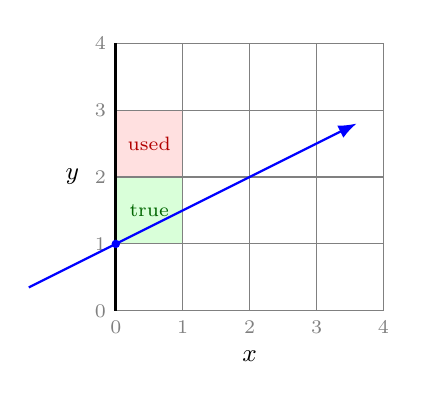
\begin{tikzpicture}[scale=0.85]
  \fill[green!15] (0,1) rectangle (1,2);
  \fill[red!12] (0,2) rectangle (1,3);
  \draw[gray] (0,0) grid (4,4);
  \draw[very thick] (0,0) -- (0,4);
  \foreach \y in {0,...,4} \node[left,gray] at (0,\y) {\scriptsize $\y$};
  \foreach \x in {0,...,4} \node[below,gray] at (\x,0) {\scriptsize $\x$};
  \node[below] at (2,-0.45) {\small $x$};
  \node[left] at (-0.4,2) {\small $y$};
  \draw[-{Latex},thick,blue] (-1.3,0.35) -- (0,1) -- (3.6,2.8);
  \fill[blue] (0,1) circle (1.8pt);
  \node[green!40!black,font=\scriptsize] at (0.5,1.5) {true};
  \node[red!70!black,font=\scriptsize,align=center] at (0.5,2.5) {used};
\end{tikzpicture}
\caption{Case (i). Entry through the near face $x=0$ at $y=1$, moving up. The plane $y=1$ is counted
as a crossing of length zero, so after the first step the index is $j=2$ while the ray is in $j=1$.}
\end{subfigure}\hfill
\begin{subfigure}[t]{0.47\linewidth}\centering
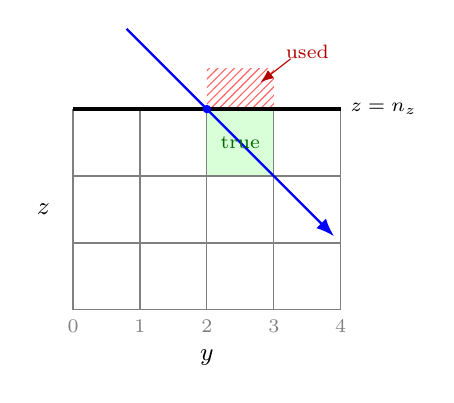
\begin{tikzpicture}[scale=0.85]
  \fill[green!15] (2,2) rectangle (3,3);
  \fill[pattern=north east lines,pattern color=red!60] (2,3) rectangle (3,3.6);
  \draw[gray] (0,0) grid (4,3);
  \draw[very thick] (0,3) -- (4,3);
  \foreach \y in {0,...,4} \node[below,gray] at (\y,0) {\scriptsize $\y$};
  \node[below] at (2,-0.45) {\small $y$};
  \node[left] at (-0.2,1.5) {\small $z$};
  \node[right,font=\scriptsize] at (4,3) {$z=n_z$};
  \draw[-{Latex},thick,blue] (0.8,4.2) -- (2,3) -- (3.9,1.1);
  \fill[blue] (2,3) circle (1.8pt);
  \node[green!40!black,font=\scriptsize] at (2.5,2.5) {true};
  \node[red!70!black,font=\scriptsize] at (3.5,3.85) {used};
  \draw[red!70!black,-{Latex}] (3.25,3.75) -- (2.8,3.4);
\end{tikzpicture}
\caption{Case (ii). Entry through the far face $z=n_z$, moving down, at a point also on the plane $y=2$.
The midpoint is the entry point and $\lfloor n_z\rfloor$ selects the voxel above the face; the $z$
crossings were computed for the voxel below.}
\end{subfigure}
\caption{\label{fig:cases}The two cases of Proposition~\ref{prop:jacobs}, in 2D sections.}
\end{figure}

\paragraph{Frequency.} The rays of Proposition~\ref{prop:jacobs} form a set of measure zero, and for a
generic geometry no ray lies on it exactly. In TIGRE's default cone-beam geometry ($256^3$ voxels, a
$256^2$ detector, 360 angles), not one of the 23.6 million rays of the whole image satisfies the condition
in exact arithmetic. Two things nevertheless put rays on it in practice. First, floating point turns the set
into a band: an entry point within rounding of a grid edge behaves as if it were on it, and so does a
comparison such as $\alpha_{min}=\alpha_{z\,min}$ in Eq.~\eqref{eq:limneg} that rounding decides the other
way. The band is about one unit in the last place of the coordinates wide, $\sim10^{-5}$ voxels, and in the
same geometry 372 rays have an entry point within one such unit of a failing edge, about one in 60\,000, in
line with the 424 wrong rays observed (Section~\ref{sec:res-correct}). Second, geometries aligned with the
grid can place rays on the set exactly. When the image is split into slabs, the slab faces are an integer
number of voxels from the plane of the source, and at angles that are multiples of $90^\circ$ the detector
axes are parallel to the image axes; the coordinates of entry points on a slab face are then rational
numbers with small denominators, often integers. Split into three slabs, the same geometry has 1\,074 rays
that satisfy the condition exactly, all at $0^\circ$, $90^\circ$, $180^\circ$ and $270^\circ$, in addition to
the floating-point band. Splitting also multiplies the opportunities: a whole image is entered once per ray,
whereas a ray crossing $S$ slabs enters $S$ of them. Splitting is therefore not the cause of \#859, but it is
what made it frequent.

In short, exact hits are an edge case of symmetric, grid-aligned geometries, which a calibrated scanner
geometry will practically never produce. The floating-point band, however, does not depend on the geometry:
in single precision, a small fraction of rays, of the order of $10^{-5}$, lies within rounding of the set in
any geometry, and each of them is integrated one voxel off for the rest of its path.

\begin{remark}
Siddon's original algorithm is not affected: every segment gets its own midpoint,
Eq.~\eqref{eq:midpoint}, and the segment that follows a zero-length one has a midpoint inside its voxel
again. The inconsistency is introduced by taking a single midpoint, Eq.~\eqref{eq:jstart}, and then only
incrementing.
\end{remark}

\subsection{Accumulation of rounding errors}
\label{sec:drift}

In floating point the update of Eq.~\eqref{eq:jacobs} is $\alpha_x\gets\fl(\alpha_x+\alpha_{xu})$, which
adds a small number to a large one. In voxel coordinates $\|\mathbf{r}\|$ is of the order of the
source--detector distance in voxels, e.g.\ $\approx3000$ for a $512^3$ image of 0.5\,mm voxels and a
source--detector distance of 1536\,mm, so one voxel step changes $\alpha$ by
$\alpha_{xu}=1/|r_x|\gtrsim3\times10^{-4}$, while inside the image $\alpha$ is about DSO/DSD $\approx0.65$.
Each addition is rounded to a multiple of $\mathrm{ulp}(0.65)\approx6\times10^{-8}$, an error of up to
$\sim10^{-4}$ of a voxel step. After $m$ steps the computed crossing has accumulated up to $m$ such errors,
and typically $\sim\sqrt m$ of them; at $512^3$, with a few hundred steps per axis, crossings end up
$10^{-3}$ to $10^{-2}$ of a voxel step from their exact position.

A boundary displaced by $\delta\alpha$ moves a length $\|\mathbf r\|_\Delta\,\delta\alpha$ from one voxel to
its neighbour, so by Eq.~\eqref{eq:sum} the error in $d_{ray}$ is
\begin{equation}
\delta d_{ray}\approx\|\mathbf r\|_\Delta\sum_m\delta\alpha_m\big(\I(\mathbf v_m)-\I(\mathbf v_{m+1})\big),
\end{equation}
proportional to the jumps of the image between neighbouring voxels: largest for rough images, small for
smooth ones. Evaluating each crossing directly from Eq.~\eqref{eq:alphax}, as Siddon did, gives an error
of a few roundoffs of $\alpha$ per crossing, independent of its position along the ray. The incremental
update is a speed optimisation that trades this for one addition instead of a multiplication and a
division.

\section{A consistent traversal for GPUs}
\label{sec:new}

\subsection{Consistent initialisation and direct crossings}

The first voxel is the one the ray is in just after entering. On a plane, the direction of travel
decides the side:
\begin{equation}
i_0=\begin{cases}\lfloor e_x\rfloor & r_x\ge0\\ \lceil e_x\rceil-1 & r_x<0\end{cases},\qquad
i_0\gets\min(\max(i_0,0),\,n_x-1), \label{eq:start}
\end{equation}
and likewise for $j_0,k_0$. This replaces Eq.~\eqref{eq:jstart}. It is the initialisation of Amanatides and
Woo's traversal~\cite{amanatides1987fast}, written out for entry points on planes, where the direction of
travel decides the side. The clamp only absorbs entry points that rounding places a hair outside the image.
The next crossing along each axis is the face of the current voxel ahead of the ray, computed from its plane
with Eq.~\eqref{eq:alphax}, as in Siddon's original formulation~\cite{siddon1985fast}: $\alpha_x(i+1)$ for
$r_x>0$ and $\alpha_x(i)$ for $r_x<0$. This replaces Eqs.~\eqref{eq:limpos}--\eqref{eq:first} and the
incremental update in Eq.~\eqref{eq:jacobs}. Deriving the crossings from the current voxel, rather than from
separately computed plane limits, is also what several CPU implementations do
(Section~\ref{sec:discussion}); it is what makes the first voxel and the crossings agree.

\begin{lemma}\label{lem:consistent}
In exact arithmetic, the traversal defined by Eq.~\eqref{eq:start}, the crossings $\alpha_x(i+1)$ or
$\alpha_x(i)$ of the current voxel, and the update of Eq.~\eqref{eq:jacobs} without the increment
$\alpha_{xu}$, computes Eq.~\eqref{eq:sum} exactly for every ray with $\alpha_{min}<\alpha_{max}$.
\end{lemma}

\begin{proof}[Proof sketch]
For every axis, $\mathbf{p}(\alpha)$ lies in the slab $[i_0,i_0+1)$ (resp.\ $(i_0,i_0+1]$ for $r_x<0$) for
$\alpha$ just above $\alpha_{min}$, by construction of Eq.~\eqref{eq:start}. The crossing computed for
the current index is therefore the next plane the ray meets along that axis, and crossing it moves the
ray into the slab of the updated index. By induction, the index always names the voxel the ray is in,
and the crossings are visited in increasing order, so the segments are those of Eq.~\eqref{eq:sum};
segments of zero length (edges and corners) contribute nothing.
\end{proof}

The loop ends when the next crossing reaches $\alpha_{max}$, the last segment ending exactly at
$\alpha_{max}$, so $N_p$ and the plane limits of Eqs.~\eqref{eq:limpos}--\eqref{eq:limneg} are no longer
needed. In floating point, a step limit $n_x+n_y+n_z+3$ guarantees termination even if rounding never lets
a crossing reach $\alpha_{max}$.

\subsection{What is costly on a GPU}
\label{sec:gpucost}

Siddon's and Jacobs' algorithms minimise arithmetic, the appropriate measure on the scalar processors for
which they were designed. A GPU executes threads in warps of 32 that issue each instruction
together~\cite{cudaguide}, and its costs differ in four ways that matter here. None of them is specific to
ray tracing; they are the standard considerations of GPU programming, applied to this loop.

A texture fetch takes tens to hundreds of cycles, and independent arithmetic issued while it is in flight
is nearly free: the memory reads, not the arithmetic, set the pace. When the threads of a warp take
different branches, the warp executes each branch in turn with the other threads masked. Neighbouring rays
cross similar planes, but not at the same step: at a given iteration one ray crosses an $x$ plane while its
neighbour crosses a $y$ plane. In the original kernel the texture fetch was inside each of the three
branches of Eq.~\eqref{eq:jacobs}, so a warp could issue up to three fetches per step.

Integer--float conversions have a fraction of the throughput of a fused multiply--add. The texture is
addressed with floating-point coordinates, so the original kernel converted three indices for every fetch,
and it updated the index in floating point, $i=\fl(i+i_u)$, converting back. In TIGRE the indices were
\texttt{unsigned long}, 64-bit on Linux, and 64-bit conversions proved far slower still
(Section~\ref{sec:res-speed}); the type of the indices is easy to overlook in any implementation.

Finally, an FMA costs the same as an addition. Evaluating Eq.~\eqref{eq:alphax} as
$\fl(b\,r_x^{-1}+o_x)$, with $r_x^{-1}=1/r_x$ and $o_x=-p_{x1}/r_x$ computed once per ray, costs one FMA, as
much as the addition in Eq.~\eqref{eq:jacobs}. Computing crossings directly is therefore not more expensive
than accumulating them.

\subsection{Implementation}

Two choices follow. The texture fetch is placed at the start of each step, identical for all threads,
and only the update of the axis crossed is in the branch. And after the initialisation the voxel is kept
as the coordinates of its centre, $c_x=i+\tfrac12$, which is what the texture fetch takes: the loop needs
no conversion. Centres are exact in single precision for fewer than $2^{23}$ voxels per axis. The face
ahead of the voxel is at $c_x+h_x$, $h_x=s_x/2$, so the next crossing is
\begin{equation}
\alpha_x=\fl\big((c_x+h_x)\,r_x^{-1}+o_x\big). \label{eq:fma}
\end{equation}
Figure~\ref{fig:diagram}(b) shows these variables. Algorithm~\ref{alg:both} sets the new traversal next to
Jacobs', with the lines that differ highlighted, and Appendix~\ref{app:code} gives the CUDA code.

\begin{figure}[t]
\centering
\begin{subfigure}[t]{0.49\linewidth}\centering
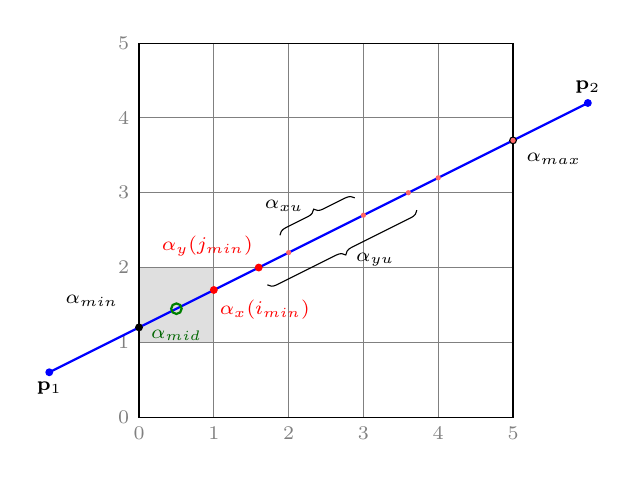
\begin{tikzpicture}[scale=0.95,>={Latex[length=2mm]}]
  \fill[gray!25] (0,1) rectangle (1,2);
  \draw[gray] (0,0) grid (5,5);
  \draw (0,0) rectangle (5,5);
  \foreach \x in {0,...,5} \node[below,gray,font=\scriptsize] at (\x,0) {$\x$};
  \foreach \y in {0,...,5} \node[left,gray,font=\scriptsize] at (0,\y) {$\y$};
  \draw[blue,thick] (-1.2,0.6) -- (6,4.2);
  \fill[blue] (-1.2,0.6) circle (1.5pt) node[below,black,font=\scriptsize] {$\mathbf p_1$};
  \fill[blue] (6,4.2) circle (1.5pt) node[above,black,font=\scriptsize] {$\mathbf p_2$};
  % entry and exit
  \fill (0,1.2) circle (1.5pt);
  \node[font=\scriptsize,anchor=east] at (-0.15,1.55) {$\alpha_{min}$};
  \fill (5,3.7) circle (1.5pt);
  \node[font=\scriptsize,anchor=west] at (5.05,3.45) {$\alpha_{max}$};
  % first crossings
  \fill[red] (1,1.7) circle (1.5pt);
  \node[red,font=\scriptsize,anchor=north west] at (0.95,1.7) {$\alpha_x(i_{min})$};
  \fill[red] (1.6,2) circle (1.5pt);
  \node[red,font=\scriptsize,anchor=south east] at (1.65,2.02) {$\alpha_y(j_{min})$};
  % midpoint
  \draw[green!50!black,thick] (0.5,1.45) circle (2pt);
  \node[green!40!black,font=\scriptsize,anchor=north] at (0.5,1.3) {$\alpha_{mid}$};
  % alpha_xu and alpha_yu
  \draw[decorate,decoration={brace,amplitude=3pt,raise=7pt}] (2,2.2) -- (3,2.7)
     node[midway,above left=8pt,font=\scriptsize,inner sep=0pt] {$\alpha_{xu}$};
  \draw[decorate,decoration={brace,amplitude=3pt,mirror,raise=7pt}] (1.6,2) -- (3.6,3)
     node[midway,below right=8pt,font=\scriptsize,inner sep=0pt] {$\alpha_{yu}$};
  \foreach \x in {2,3,4,5} \fill[red!60] (\x,{1.2+0.5*\x}) circle (1pt);
  \fill[red!60] (3.6,3) circle (1pt);
\end{tikzpicture}
\caption{Jacobs. The first crossing on each axis (red) comes from the plane limits,
Eqs.~\eqref{eq:limpos}--\eqref{eq:first}; the first voxel (grey) from the midpoint $\alpha_{mid}$ of the
first segment, Eq.~\eqref{eq:jstart}. Later crossings are found by adding $\alpha_{xu}$ or $\alpha_{yu}$,
Eq.~\eqref{eq:jacobs}.}
\end{subfigure}\hfill
\begin{subfigure}[t]{0.49\linewidth}\centering
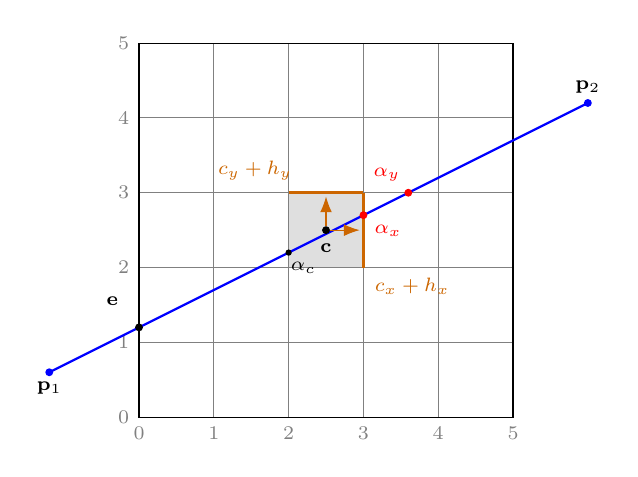
\begin{tikzpicture}[scale=0.95,>={Latex[length=2mm]}]
  \fill[gray!25] (2,2) rectangle (3,3);
  \draw[gray] (0,0) grid (5,5);
  \draw (0,0) rectangle (5,5);
  \foreach \x in {0,...,5} \node[below,gray,font=\scriptsize] at (\x,0) {$\x$};
  \foreach \y in {0,...,5} \node[left,gray,font=\scriptsize] at (0,\y) {$\y$};
  \draw[blue,thick] (-1.2,0.6) -- (6,4.2);
  \fill[blue] (-1.2,0.6) circle (1.5pt) node[below,black,font=\scriptsize] {$\mathbf p_1$};
  \fill[blue] (6,4.2) circle (1.5pt) node[above,black,font=\scriptsize] {$\mathbf p_2$};
  \fill (0,1.2) circle (1.5pt);
  \node[font=\scriptsize,anchor=east] at (-0.15,1.55) {$\e$};
  % current voxel centre and faces ahead
  \fill (2.5,2.5) circle (1.5pt);
  \node[font=\scriptsize,anchor=north] at (2.5,2.45) {$\mathbf c$};
  \draw[orange!80!black,very thick] (3,2) -- (3,3);
  \draw[orange!80!black,very thick] (2,3) -- (3,3);
  \draw[->,orange!80!black] (2.55,2.5) -- (2.95,2.5);
  \draw[->,orange!80!black] (2.5,2.55) -- (2.5,2.95);
  \node[orange!80!black,font=\scriptsize] at (3.65,1.75) {$c_x+h_x$};
  \node[orange!80!black,font=\scriptsize] at (1.55,3.3) {$c_y+h_y$};
  % crossings of the faces ahead
  \fill[red] (3,2.7) circle (1.5pt);
  \node[red,font=\scriptsize,anchor=north west] at (3.02,2.7) {$\alpha_x$};
  \fill[red] (3.6,3) circle (1.5pt);
  \node[red,font=\scriptsize,anchor=south east] at (3.62,3.02) {$\alpha_y$};
  \fill (2,2.2) circle (1.2pt);
  \node[font=\scriptsize,anchor=north west] at (1.9,2.2) {$\alpha_c$};
\end{tikzpicture}
\caption{Revised. The first voxel comes from the entry point $\e$ and the direction of travel,
Eq.~\eqref{eq:start}. The voxel is kept as its centre $\mathbf c$; each crossing is computed from the face
ahead of it (orange), $\alpha_x=\fl\big((c_x+h_x)r_x^{-1}+o_x\big)$, Eq.~\eqref{eq:fma}.}
\end{subfigure}
\caption{\label{fig:diagram}Variables of the two traversals, in 2D, for the same ray. Adapted from the
diagram of~\cite{biguri2017}.}
\end{figure}

\begin{algorithm}[t]
\caption{\label{alg:both}Jacobs' traversal, Eqs.~\eqref{eq:limpos}--\eqref{eq:jacobs} (left), and the
revised one (right), for one ray after $\alpha_{min}$ and $\alpha_{max}$ are computed. Only the $x$ branch
of the update is written out. Highlighted lines differ. $\alpha_d=\infty$ for an axis with $r_d=0$.}
\begin{minipage}[t]{0.47\linewidth}
\begin{algorithmic}[1]
\State $i_{min},i_{max},\dots$ \Comment{Eqs.~\eqref{eq:limpos}--\eqref{eq:limneg}}
\State $\alpha_d\gets\alpha_d(d_{min})$ or $\alpha_d(d_{max})$ \Comment{Eq.~\eqref{eq:first}}
\State $N_p\gets\sum_d(d_{max}-d_{min}+1)$
\State $(i,j,k)\gets\lfloor\mathbf p(\alpha_{mid})\rfloor$ \Comment{Eq.~\eqref{eq:jstart}}
\State $\alpha_c\gets\alpha_{min}$, $d_{ray}\gets0$
\For{$N_p$ steps}
  \If{$\alpha_x\le\min(\alpha_y,\alpha_z)$}
    \State $d_{ray}\mathrel{+}=(\alpha_x-\alpha_c)\,\I(i,j,k)$
    \State $i\gets i+i_u$; $\alpha_c\gets\alpha_x$
    \State $\alpha_x\gets\alpha_x+\alpha_{xu}$
  \ElsIf{$\alpha_y\le\alpha_z$} \dots
  \Else\ \dots
  \EndIf
\EndFor
\State \Return $\|\mathbf r\|_\Delta\,d_{ray}$
\end{algorithmic}
\end{minipage}\hfill
\begin{minipage}[t]{0.51\linewidth}
\begin{algorithmic}[1]
\State \chg{$(c_x,c_y,c_z)\gets(i_0,j_0,k_0)+\tfrac12$} \Comment{Eq.~\eqref{eq:start}}
\State \chg{$h_d\gets s_d/2$, $r_d^{-1}\gets1/r_d$, $o_d\gets-p_{d1}r_d^{-1}$}
\State \chg{$\alpha_d\gets\fl\big((c_d+h_d)r_d^{-1}+o_d\big)$} \Comment{Eq.~\eqref{eq:fma}}
\State
\State $\alpha_c\gets\alpha_{min}$, $d_{ray}\gets0$
\For{\chg{at most $n_x+n_y+n_z+3$} steps}
  \State \chg{$\alpha_n\gets\min(\alpha_x,\alpha_y,\alpha_z)$}
  \State \chg{$d_{ray}\mathrel{+}=\big(\min(\alpha_n,\alpha_{max})-\alpha_c\big)\,\I(\mathbf c)$}
  \State \chg{\textbf{if} $\alpha_n\ge\alpha_{max}$ \textbf{break}}
  \If{$\alpha_x=\alpha_n$}
    \State \chg{$c_x\gets c_x+s_x$}; $\alpha_c\gets\alpha_x$
    \State \chg{$\alpha_x\gets\fl\big((c_x+h_x)r_x^{-1}+o_x\big)$}
  \ElsIf{$\alpha_y=\alpha_n$} \dots
  \Else\ \dots
  \EndIf
\EndFor
\State \Return $\|\mathbf r\|_\Delta\,d_{ray}$
\end{algorithmic}
\end{minipage}
\end{algorithm}

The two loops have the same shape. The differences are where the voxel is read, now once per step outside
the branch; how the crossing is advanced, now evaluated from the plane instead of accumulated; how the
voxel is held, now as a floating-point centre; and how the loop ends, now at $\alpha_{max}$ instead of after
$N_p$ steps. Reading the voxel before the branch requires the length of the segment before knowing which
axis is crossed, hence $\alpha_n$, and the last segment is clipped at $\alpha_{max}$.

\paragraph{Rounding.} Each crossing carries the error of one evaluation of Eq.~\eqref{eq:fma}: the
rounding of the FMA, and those of $r_x^{-1}$ and $o_x$. The latter two are common to all crossings of the
ray, so they shift and scale them together by a relative $\sim10^{-7}$, which is equivalent to an equally
small change of geometry and does not affect how length is shared between voxels. No error grows with
the number of steps.

\paragraph{Indices.} The integer indices exist only in Eq.~\eqref{eq:start}, as 32-bit signed integers:
signed because $\lceil e_x\rceil-1$ can be $-1$ before the clamp. (The original kernel converted such
values to an unsigned type, which is undefined for negative values; on the GPU it produced the
out-of-image first voxel of case (ii).)

\paragraph{Parallel beam.} The same traversal applies unchanged to parallel beam, where each ray has its
own source point; an axis with $r_d=0$ is never crossed. TIGRE's parallel-beam kernel had the same loop as
its cone-beam one and received the same change.

\subsection{Operation counts}
\label{sec:flops}

Siddon designed his algorithm to minimise floating-point operations, and Jacobs' variant reduces them
further. Table~\ref{tab:flops} counts the operations per crossing of the three formulations, as written
above (not from machine code). Jacobs' step needs three arithmetic operations, the subtraction and the
multiply--add of the accumulation and the increment of $\alpha_x$, against about eight for Siddon's merge,
midpoint and voxel index, plus three float-to-integer conversions. The revised step has the same
arithmetic as Jacobs': the increment becomes an FMA, which costs the same, and the integer increment of the
index becomes a floating-point one. What it adds are two or three comparisons: the minimum $\alpha_n$, the
clamp to $\alpha_{max}$ and the termination test, which replace Jacobs' integer step counter. In operation
counts, then, the revised step is marginally more expensive than Jacobs' and about half the cost of
Siddon's. On a GPU these counts do not decide the time (Section~\ref{sec:gpucost}): the revised step is
faster because it issues one memory read per warp and no conversions (Section~\ref{sec:res-speed}).

\begin{table}[h]
\centering
\caption{\label{tab:flops}Operations per plane crossing, in the loop, excluding the per-ray setup.
FMA counts as one operation. ``GPU'': the conversions needed to address a texture with integer indices,
as in the original kernel.}
\begin{tabular}{lccc}
\toprule
& Siddon (merge, midpoint) & Jacobs & revised\\
\midrule
floating-point arithmetic & $\approx8$ & 3 & 4\\
comparisons / min        & $\approx2$ & 2--3 & 5--6\\
integer operations        & --- & 1 & ---\\
float--integer conversions & 3 & 0 (3 on GPU) & 0\\
memory reads              & 1 & 1 & 1\\
\bottomrule
\end{tabular}
\end{table}

\subsection{Three issues, one traversal}
\label{sec:coupling}

The original kernel had three independent problems: an inconsistent initialisation
(Section~\ref{sec:init}), accumulated rounding errors (Section~\ref{sec:drift}), and a slow loop
(Section~\ref{sec:gpucost}). Their causes are unrelated, and each could be fixed alone
(Table~\ref{tab:coupling}). In particular the speed has nothing to do with the two flaws: moving the fetch out
of the branches and using 32-bit indices would have given Jacobs' traversal, flaws included, most of the gain
(Table~\ref{tab:variants}).

\begin{table}[h]
\centering
\caption{\label{tab:coupling}The three issues of the original kernel, their causes, and the change that
addresses each. Times are from the ablation of Section~\ref{sec:res-speed}, relative to the original kernel.}
\small
\begin{tabular}{>{\raggedright\arraybackslash}p{0.12\linewidth}>{\raggedright\arraybackslash}p{0.25\linewidth}>{\raggedright\arraybackslash}p{0.28\linewidth}>{\raggedright\arraybackslash}p{0.24\linewidth}}
\toprule
issue & cause & change & if done alone\\
\midrule
consistency & first voxel from a midpoint, Eq.~\eqref{eq:jstart}, crossings from plane limits,
Eqs.~\eqref{eq:limpos}--\eqref{eq:first} & first voxel from entry point and direction, Eq.~\eqref{eq:start};
crossings from the current voxel (Amanatides and Woo) & no measurable cost (once per ray)\\
accuracy & crossings accumulated, $\alpha_x\mathrel{+}=\alpha_{xu}$ & each crossing from its plane,
Eq.~\eqref{eq:fma} (Siddon) & 10\% slower with an integer index; free with float centres\\
speed & fetch inside the branches; integer--float conversions; 64-bit indices on Linux & one fetch before
the branch; float voxel centres; 32-bit indices & 0.55--0.74 of the time; 32-bit indices alone remove
a 5--8$\times$ slowdown on Linux\\
\bottomrule
\end{tabular}
\end{table}

The changes do interact, and this is why one traversal is the natural way to make them. Deriving the
crossings from the current voxel is what makes the initialisation consistent, and it also removes the plane
limits and $N_p$. Computing each crossing from its plane costs a multiply--add per step, but keeping the voxel
as a floating-point centre, which the speed change introduces to remove conversions, makes that multiply--add
take the place of Jacobs' addition, so the accuracy comes at no cost. Conversely, the fixes cost nothing only
in this arrangement: computing the crossings from an integer index made the loop about 10\% slower. The
result is a single loop, Algorithm~\ref{alg:both} (right), that is consistent, accurate and fast; but readers
who only want the speed of Section~\ref{sec:res-speed} can obtain most of it with the changes in the last
row of Table~\ref{tab:coupling}.

\section{Experiments}
\label{sec:results}

The experiments answer three questions, one for each claim of the previous sections. First, correctness:
does the original kernel fail on the rays predicted by Proposition~\ref{prop:jacobs}, often enough to
matter, and does the new kernel compute those rays correctly? Second, accuracy: how large is the rounding
error of the incremental update described in Section~\ref{sec:drift}, and how much does the direct
evaluation of Eq.~\eqref{eq:fma} reduce it? Third, speed: does the new traversal cost anything, and if it is
faster, which of its changes make it so?

\subsection{Setup}

All experiments use TIGRE, before and after the changes, as the implementation. Two systems were used:
Windows with an NVIDIA RTX~4070 (Ada) and CUDA~12.3, and Linux with a Quadro RTX~6000 (Turing) and
CUDA~12.5. Geometries are TIGRE's default cone-beam geometry (source--origin 1000\,mm, source--detector
1536\,mm, image 256\,mm wide, detector pixels of 0.8\,mm) at $n^3$ voxels with an $n\times n$ detector.
Accuracy was measured with a CPU emulation of the kernels in single precision, which reproduces the GPU
outputs exactly, against the same traversal evaluated in double precision. Timings compare builds of TIGRE
before and after the change in separate processes, in alternating order over several rounds (after a
warm-up on Linux), with image and projections as GPU arrays; kernel time is taken from the PyTorch profiler
and the whole call is synchronised. We report the mean ratio over rounds with a 95\% confidence interval.

\subsection{Correctness}
\label{sec:res-correct}

We first compared the original and the new kernel on the GPU for a whole $256^3$ image and 360 angles.
Of 23.6 million rays, 424 differ by more than 0.1\%, the worst by 14\%. To decide which kernel is right we
evaluated the four worst rays in double precision: in every case the double-precision value agrees with the
new kernel (for example, original 127.07, new 145.38, exact 145.38), and the single-precision emulation of
the original kernel reproduces its wrong value, so the error is in the traversal and not in the hardware.
When the same image is split into slabs, as TIGRE does when memory is short, errors grow to about 20\% on
some rays, as expected from the larger number of rays that enter a slab on a plane.

Tracing one of these rays shows case (ii) of Proposition~\ref{prop:jacobs} at work. For a $256^3$ image in
3 slabs of 86 slices, at angle 0, the ray of pixel $(v,u)=(36,158)$ enters the first slab through its top
face at $\e=(246.688,\,142.000000,\,86.000000)$, exactly on the plane $y=142$. This is the second mechanism
of Section~\ref{sec:init}: at angle 0 the face $z=86$ is 42 voxels from the plane of the source, the pixel is
$30.5$ and $-91.5$ pixels from the detector centre, and $e_y=128+42\times30.5/91.5=142$. The first $y$ crossing is at
$\alpha_{min}+1.2\times10^{-7}$, so the midpoint of Eq.~\eqref{eq:jstart} is the entry point and gives
$k=86$, outside the slab, while the $z$ crossings of Eq.~\eqref{eq:first} start at $z=85$. The slab
contributes 104.80 instead of 122.86, 15\% less.

These comparisons look at individual rays; TIGRE's test suite checks the projector as a whole. On both
systems, split and unsplit projections of a $512^3$ random image agree to $10^{-4}$ of the maximum, a test
the original kernel fails. The projector tests that check known line integrals, linearity and the agreement
between the ray--voxel and interpolated projectors pass, and projections computed from GPU arrays are
identical to those computed from host arrays. These tests cover parallel beam too, and pass with the new
parallel-beam kernel (Windows).

\subsection{Accuracy}

To isolate the rounding error from the initialisation, we compared each traversal in single precision
against itself in double precision, on 150 random rays through a $512^3$ image. We used two images, chosen
to test the prediction of Section~\ref{sec:drift} that the error of the incremental update scales with the
jumps of the image between neighbouring voxels: a rough one, with voxel values uniform in $[0,1)$, and a
smooth one, a sum of two Gaussians.

\begin{table}[h]
\centering
\caption{\label{tab:acc}Relative error of single-precision line integrals against double precision,
150 random rays through a $512^3$ image.}
\begin{tabular}{llccc}
\toprule
image & traversal & median & 95th percentile & max\\
\midrule
rough & incremental, Eq.~\eqref{eq:jacobs} & $1.1\times10^{-4}$ & $6.3\times10^{-4}$ & $1.7\times10^{-3}$\\
      & direct, Eq.~\eqref{eq:fma}        & $2.5\times10^{-6}$ & $8.1\times10^{-6}$ & $1.1\times10^{-5}$\\
\midrule
smooth & incremental & $3.2\times10^{-5}$ & $1.3\times10^{-4}$ & $2.1\times10^{-4}$\\
       & direct      & $4.4\times10^{-7}$ & $1.5\times10^{-6}$ & $2.6\times10^{-6}$\\
\bottomrule
\end{tabular}
\end{table}

Table~\ref{tab:acc} confirms both predictions. The incremental update loses three to four significant
digits, up to $1.7\times10^{-3}$ on the rough image, and about five times less on the smooth one. The
direct evaluation is 40--150 times more accurate on both, with errors of $10^{-5}$ or less, close to what
single precision allows for a sum of a few hundred terms. These errors are below the noise of measured
data, which is why they had gone unnoticed (Section~\ref{sec:discussion}); they matter when projections are
compared with each other, as in the split-versus-unsplit test, and in algorithms that rely on the operator
being reproducible.

\subsection{Speed}
\label{sec:res-speed}

The new kernel changes several things at once, and comparing it with the original only tells whether it is
faster, not why. We therefore first built an ablation, in which each variant changes one thing, and then
measured the whole change in TIGRE, which is what users see.

\paragraph{Ablation.} The kernel was copied into a standalone CUDA program with variants that each change
one aspect of the loop, run interleaved in one process with TIGRE's texture settings, launch configuration
and geometry. Since a variant can appear faster by doing less work, each variant's output is compared with
the new kernel's (Table~\ref{tab:variants}).

\begin{table}[h]
\centering
\caption{\label{tab:variants}Ablation: kernel time relative to the original kernel, standalone variants,
RTX 4070, Windows, 360 angles, median of 15--30 rounds. ``Max diff'': largest difference from the new
kernel's output, relative to its maximum. On Windows \texttt{long} is 32-bit, so the original indices are
32-bit there; the 64-bit rows correspond to the original kernel on Linux.}
\begin{tabular}{lccc}
\toprule
variant & $256^3$ & $512^3$ & max diff \\
\midrule
original                                                          & 1.00 & 1.00 & $8$--$9\times10^{-2}$\\
original, index step as an integer add                            & 1.00 & 0.99 & $8$--$9\times10^{-2}$\\
original, 64-bit indices                                          & 8.09 & 7.60 & $8$--$9\times10^{-2}$\\
one convergent fetch; incremental crossings                       & 0.71 & 0.74 & $\le2\times10^{-3}$\\
one convergent fetch; direct crossings from an integer index      & 0.80 & 0.81 & 0\\
\textbf{new}: one convergent fetch; direct crossings from float centres & \textbf{0.55} & \textbf{0.67} & 0\\
new, with 64-bit indices                                          & 5.29 & 4.69 & 0\\
\bottomrule
\end{tabular}
\end{table}

Moving the fetch out of the branches gives most of the gain, about 30\%, and keeping the voxel as
floating-point centres a further 10--15\%, by removing the conversions that computing the crossing from an
integer index would add. Doing the original index step as an integer addition changes nothing, and 64-bit
indices make any variant 5--8 times slower on this GPU. Appendix~\ref{app:sass} relates these numbers to the
machine code.

\paragraph{In TIGRE.} The standalone program leaves out everything around the kernel, so we also compared
complete builds of TIGRE, before and after the change, measuring both the kernel time and the whole
projection call, which includes memory transfers and setup. Because GPU clocks vary with temperature and
with other work, the two builds were run alternately, each in a fresh process, over several rounds, and we
report the ratio with its confidence interval (Table~\ref{tab:bench}).

\begin{table}[h]
\centering
\caption{\label{tab:bench}New against original kernel in TIGRE: time ratio, mean with 95\% confidence
interval over 4--6 rounds.}
\small\setlength{\tabcolsep}{4pt}
\begin{tabular}{lcccccc}
\toprule
& \multicolumn{4}{c}{cone beam} & \multicolumn{2}{c}{parallel beam}\\
\cmidrule(lr){2-5}\cmidrule(lr){6-7}
& \multicolumn{2}{c}{Windows, RTX 4070} & \multicolumn{2}{c}{Linux, Quadro RTX 6000} & \multicolumn{2}{c}{Windows, RTX 4070}\\
\cmidrule(lr){2-3}\cmidrule(lr){4-5}\cmidrule(lr){6-7}
image, angles & kernel & whole call & kernel & whole call & kernel & whole call\\
\midrule
$128^3$, 360 & $0.54\pm0.02$ & $0.76\pm0.06$ & $0.152\pm0.001$ & $0.24\pm0.01$ & $0.593\pm0.005$ & $0.76\pm0.06$\\
$256^3$, 360 & $0.56\pm0.02$ & $0.64\pm0.02$ & $0.158\pm0.001$ & $0.175\pm0.001$ & $0.530\pm0.008$ & $0.58\pm0.04$\\
$512^3$, 360 & $0.67\pm0.01$ & $0.69\pm0.01$ & $0.177\pm0.000$ & $0.182\pm0.001$ & $0.543\pm0.010$ & $0.57\pm0.03$\\
$768^3$, 180 & $0.69\pm0.01$ & $0.74\pm0.01$ & --- & --- & $0.506\pm0.012$ & $0.55\pm0.01$\\
\bottomrule
\end{tabular}
\end{table}

For cone beam, the new kernel takes 54--69\% of the original's time on Windows and 15--18\% on Linux (at
$512^3$, 2054\,ms of kernel time become 364\,ms), consistent with the 64-bit rows of the ablation. It was
faster in every round for every size. The gain is smaller for larger images, plausibly because more texture
reads miss the cache and the kernel becomes more memory-bound; we did not verify this. For parallel beam the
new kernel takes 51--59\% of the original's time, and its gain does not shrink with image size; TIGRE's
original parallel-beam kernel had extra corrections in its initialisation.

\section{Discussion}
\label{sec:discussion}

\paragraph{Why these problems went unnoticed.} The inconsistent initialisation affects, in any geometry, a
fraction of rays of the order of $10^{-5}$ (one in 50\,000 in our example), each wrong by an amount comparable
to the difference between neighbouring voxels, and scattered across projections: invisible in a
reconstruction. The drift affects every ray, but by $10^{-4}$--$10^{-3}$, below the noise of measured data.
Neither changes a reconstruction in practice; what they break is consistency. Both became visible only when
projections of the same image computed in slabs and in one piece were compared, which changes where the
traversal starts and so where the accumulation restarts.

\paragraph{Generality.} Proposition~\ref{prop:jacobs} concerns the incremental algorithm as published, not
TIGRE's code: any implementation that initialises with a single midpoint, Eq.~\eqref{eq:jstart}, and then
only increments shares it, on CPU or GPU, in single or double precision. The drift affects any implementation
that accumulates crossings in single precision. Double precision is not a good alternative on GPUs, where it
runs at a small fraction of the single-precision rate, and the direct evaluation already achieves an error of
about $10^{-5}$. The arrangement around one convergent fetch is specific to SIMT hardware.

\paragraph{Related implementations.} Appendix~\ref{app:related} summarises how the open-source
implementations we examined deal with these issues. Each ingredient of Section~\ref{sec:new} exists
elsewhere: the consistent initialisation in Amanatides and Woo and in several CPU codes, the direct
evaluation of crossings in Siddon's method. To the best of our knowledge, none of the implementations we
examined combines a consistent initialisation, crossings computed without accumulation at the cost of
Jacobs' traversal, and a loop arranged for SIMT execution. We did not survey implementations systematically,
and did not benchmark against them.

\paragraph{Rays inside a plane.} A ray that lies in a plane between voxels ($r_b=0$, $e_b\in\mathbb Z$) has an
ambiguous line integral. STIR traces it twice, half a voxel to each side, and averages. Our traversal, like
Siddon's midpoint rule, takes the voxel on the positive side. This is a modelling choice rather than an
error, but a symmetric treatment may be preferable for geometries that produce many such rays.

\paragraph{Limitations.} Speed was measured on two GPUs of two generations, accuracy by emulation on 150 rays
per image, and correctness in exact arithmetic on a small grid; the parallel-beam kernel was timed on Windows
only. We did not study backprojection: TIGRE's backprojectors are voxel-driven and do not use this traversal,
but a ray-driven matched backprojector built on Jacobs' traversal would inherit both flaws.

\section{Conclusion}

The incremental form of Siddon's algorithm, as published by Jacobs et al.\ and commonly implemented, has two
flaws: an initialisation that is inconsistent for an exactly characterised set of rays, and, in single
precision, rounding errors that accumulate along the ray. Both have known remedies, the initialisation of
Amanatides and Woo and the direct evaluation of crossings of Siddon's original method. This note shows how to
combine them on a GPU without extra cost, by organising the step around one convergent memory read, with
floating-point voxel centres and 32-bit indices. In TIGRE the revised projector is consistent for every ray,
about 100 times more accurate, and 1.4--6.5 times faster, depending on the platform; most of the speed comes
from the GPU arrangement, not from the algorithm.

\section*{Code availability}
The implementation is part of TIGRE, \url{https://github.com/CERN/TIGRE}, from pull request \#865. The cone-beam kernel is in
\path{Common/CUDA/Siddon_projection.cu} and the parallel-beam kernel in \path{Common/CUDA/Siddon_projection_parallel.cu}.

\section*{Author contributions}
A.~Biguri: conceptualisation, direction, testing on hardware, review and editing. Claude (Anthropic, a large
language model): investigation, analysis, implementation, emulations, benchmarks and the first draft of this
note, under A.~Biguri's direction.

\begin{thebibliography}{99}
\bibitem{siddon1985fast} R.~L.~Siddon, ``Fast calculation of the exact radiological path for a
three-dimensional CT array,'' \emph{Medical Physics} 12(2):252--255, 1985.
\bibitem{jacobs1998fast} F.~Jacobs, E.~Sundermann, B.~De Sutter, M.~Christiaens, I.~Lemahieu, ``A fast
algorithm to calculate the exact radiological path through a pixel or voxel space,'' \emph{Journal of
Computing and Information Technology} 6(1):89--94, 1998.
\bibitem{amanatides1987fast} J.~Amanatides, A.~Woo, ``A fast voxel traversal algorithm for ray tracing,''
\emph{Eurographics '87}, 1987.
\bibitem{tigre2016} A.~Biguri, M.~Dosanjh, S.~Hancock, M.~Soleimani, ``TIGRE: a MATLAB-GPU toolbox for CBCT
image reconstruction,'' \emph{Biomedical Physics \& Engineering Express} 2(5):055010, 2016.
doi:10.1088/2057-1976/2/5/055010.
\bibitem{tigre2020multigpu} A.~Biguri, R.~J.~Lindroos, R.~Bryll, H.~Towsyfyan, H.~Deyhle, I.~Harrane,
R.~Boardman, M.~Mavrogordato, M.~Dosanjh, S.~Hancock, T.~Blumensath, ``Arbitrarily large tomography with
iterative algorithms on multiple GPUs using the TIGRE toolbox,'' \emph{Journal of Parallel and Distributed
Computing} 146:52--63, 2020. doi:10.1016/j.jpdc.2020.07.004.
\bibitem{tigre2025v3} A.~Biguri, T.~Sadakane, R.~Lindroos, Y.~Liu, M.~Sabat\'e Landman, Y.~Du, M.~Lohvithee,
S.~Kaser, S.~Hatamikia, R.~Bryll, E.~Valat, S.~Wonglee, T.~Blumensath, C.-B.~Sch\"onlieb, ``TIGRE v3: efficient
and easy to use iterative computed tomographic reconstruction toolbox for real datasets,''
\emph{Engineering Research Express} 7(1):015011, 2025. doi:10.1088/2631-8695/adbb3a.
\bibitem{biguri2017} A.~Biguri, \emph{Iterative Reconstruction and Motion Compensation in Computed Tomography
on GPUs}, PhD thesis, University of Bath, 2017. \url{https://github.com/AnderBiguri/PhDThesis}.
\bibitem{higham2002} N.~J.~Higham, \emph{Accuracy and Stability of Numerical Algorithms}, 2nd ed., SIAM, 2002.
\bibitem{itktpr} Insight Toolkit (ITK), \path{SiddonJacobsRayCastInterpolateImageFunction}, module
TwoProjectionRegistration (originally J.~Wu, \emph{Insight Journal}, publication 784), now in \path{Modules/Registration/TwoProjectionRegistration},
\url{https://github.com/InsightSoftwareConsortium/ITK}.
\bibitem{reg23} G.~Fattori, \path{itkgSiddonJacobsRayCastInterpolateImageFunction}, reg23Topograms, Paul
Scherrer Institut, \url{https://gitea.psi.ch/fattori_g/reg23Topograms}.
\bibitem{pyradplan} pyRadPlan, \texttt{pyRadPlan.raytracer.\_siddon},
\url{https://pyradplan.readthedocs.io}.
\bibitem{joseph1982} P.~M.~Joseph, ``An improved algorithm for reprojecting rays through pixel images,''
\emph{IEEE Transactions on Medical Imaging} 1(3):192--196, 1982.
\bibitem{astra2016} W.~van~Aarle, W.~J.~Palenstijn, J.~Cant, E.~Janssens, F.~Bleichrodt, A.~Dabravolski,
J.~De~Beenhouwer, K.~J.~Batenburg, J.~Sijbers, ``Fast and flexible X-ray tomography using the ASTRA toolbox,''
\emph{Optics Express} 24(22):25129--25147, 2016.
\bibitem{rtk2014} S.~Rit, M.~Vila~Oliva, S.~Brousmiche, R.~Labarbe, D.~Sarrut, G.~C.~Sharp, ``The Reconstruction
Toolkit (RTK), an open-source cone-beam CT reconstruction toolkit based on the Insight Toolkit (ITK),''
\emph{Journal of Physics: Conference Series} 489:012079, 2014.
\bibitem{parallelproj} parallelproj, \url{https://github.com/gschramm/parallelproj}.
\bibitem{tomopy2014} D.~G\"ursoy, F.~De~Carlo, X.~Xiao, C.~Jacobsen, ``TomoPy: a framework for the analysis of
synchrotron tomographic data,'' \emph{Journal of Synchrotron Radiation} 21(5):1188--1193, 2014.
\bibitem{stir2012} K.~Thielemans, C.~Tsoumpas, S.~Mustafovic, T.~Beisel, P.~Aguiar, N.~Dikaios, M.~W.~Jacobson,
``STIR: software for tomographic image reconstruction release 2,'' \emph{Physics in Medicine and Biology}
57(4):867--883, 2012.
\bibitem{tomograpy} TomograPy, \url{https://github.com/nbarbey/TomograPy}.
\bibitem{plastimatch} plastimatch, \url{https://gitlab.com/plastimatch/plastimatch}.
\bibitem{leap} LEAP, LivermorE AI Projector for computed tomography, \url{https://github.com/llnl/LEAP}.
\bibitem{cudaguide} NVIDIA, \emph{CUDA C++ Programming Guide}, sections on SIMT architecture and arithmetic
instruction throughput.
\end{thebibliography}

\appendix
\section{CUDA code}
\label{app:code}

Cone-beam kernel, \texttt{Common/CUDA/Siddon\_projection.cu}, after $\alpha_{min}$ (\texttt{am}) and
$\alpha_{max}$ (\texttt{aM}) are computed:
\begin{lstlisting}
int i=(ray.x<0.0f)? (int)ceilf(pX)-1 : (int)floorf(pX);      // Eq. (start); j, k alike
i=(i<0)? 0 : ((i>(int)geo.nVoxelX-1)? (int)geo.nVoxelX-1 : i);
float cX=(float)i+0.5f;                                      // voxel centre
float sX=(ray.x<0.0f)? -1.0f : 1.0f;  float hX=0.5f*sX;      // direction, face offset
float rX=(ray.x!=0.0f)? 1.0f/ray.x : 0.0f;  float oX=-source.x*rX;
float ax=(ray.x!=0.0f)? fmaf(cX+hX,rX,oX) : INFINITY;        // next x crossing
// ... same for y, z ...
float ac=am, sum=0.0f;
const int maxsteps=(int)geo.nVoxelX+(int)geo.nVoxelY+(int)geo.nVoxelZ+3;
for (int step=0; step<maxsteps; step++){
    float aminc=fminf(fminf(ax,ay),az);
    sum+=(fminf(aminc,aM)-ac)*tex3D<float>(tex, cX, cY, cZ);  // one fetch, all threads
    if (aminc>=aM) break;
    if (ax==aminc){      cX+=sX; ac=ax; ax=fmaf(cX+hX,rX,oX); }
    else if(ay==aminc){  cY+=sY; ac=ay; ay=fmaf(cY+hY,rY,oY); }
    else{                cZ+=sZ; ac=az; az=fmaf(cZ+hZ,rZ,oZ); }
}
detector[idx]=sum*maxlength;
\end{lstlisting}


\section{Machine code of the ablation variants}
\label{app:sass}

The machine code (sm\_89) explains the ablation of Table~\ref{tab:variants}. The original loop, unrolled four
times by the compiler, has 220 instructions for four steps, 12 of them texture fetches (one in each branch);
the restructured loop has 43 instructions per step and one fetch. Computing the crossing from an integer index
costs 49 instructions per step, six of them conversions, which keeping the voxel as floating-point centres
removes. Doing the original index step as an integer addition changes nothing because the conversions it saves
are not on the critical path while the fetch is divergent. The slowdown with 64-bit indices is most likely due
to 64-bit integer--float conversions taking a slow path; we did not isolate this further.

\section{Related implementations}
\label{app:related}

We read the ray--voxel code of several open-source packages for
tomography and registration. Many use other projection models, such as Joseph's
interpolation~\cite{joseph1982} (RTK~\cite{rtk2014}, parallelproj~\cite{parallelproj}, and ASTRA's 3D GPU
projectors~\cite{astra2016}), and are not concerned here. Of those that compute exact intersection lengths,
TomoPy~\cite{tomopy2014} and vectorised codes such as pyRadPlan~\cite{pyradplan} implement Siddon's original
method: every crossing is computed directly and each segment gets its own midpoint, so they are immune to
Proposition~\ref{prop:jacobs} and have no drift, at about twice the arithmetic per crossing of the
incremental form and with per-ray storage for the merge. STIR~\cite{stir2012}, TomograPy~\cite{tomograpy} and
plastimatch~\cite{plastimatch} use the incremental traversal but derive the crossings from the faces of the
first voxel, as Amanatides and Woo do, so their initialisation is consistent; they then accumulate the
crossings, or the distances to them, and so have the drift of Section~\ref{sec:drift} (in single precision
for STIR and TomograPy), and some add tolerances or explicit branches for ties. LEAP~\cite{leap} avoids a
traversal altogether: it steps through the image slice by slice along the dominant axis and computes the
exact lengths in the at most four voxels each slice can contain, with more arithmetic and memory reads per
voxel but no data-dependent branching; its positions are also accumulated. The Siddon--Jacobs ray caster of
ITK's TwoProjectionRegistration module~\cite{itktpr} takes the first voxel as the floor of the entry point
whatever the direction of travel, so rays that enter on a plane take the zero-length step of case~(i), and
it advances the voxel index before reading the voxel, so each segment is credited to the next voxel along
the ray and the first segment is lost; codes derived from it add special cases and tolerances for rays
aligned with the grid~\cite{reg23}.

\end{document}
